\documentclass[12px]{article}

\title{Lezione 18 Metodi Numerici}
\date{2026-05-15}
\author{Federico De Sisti}

\input{../../setup.tex}

\begin{document}
	\maketitle
	\newpage
	\subsection{Metodi LMM}
	\subsubsection{Ricorda}
	Ricordiamo la forma generale
	\[
		u_{n+1} = \sum^{p}_{j=0}a_ju_{n-j} + h \sum^{p}_{j=-1}b_jf_{n-j} \ \ \ \ n\geq p \ \ u_0,\ldots,u_p \ \  \text{ dati}
	.\] 
	$\displaystyle\rho(r) = r^{p+1} - \sum^{p}_{j=0}a_jr^{p - j}$ primo polinomio caratteristico\\
	$\displaystyle\sigma(r) = \sum^{p}_{j=-1}b_jr^{p-j}$ secondo polinomio caratteristico\\
	$P(r) = \rho(r) - h\lambda \sigma(r)$ polinomio caratteristico se $f = \lambda y$ \\
	Le radici $r_j$ di $\rho(r)=0 , j = 0,\ldots p$ sono soluzioni,\\ 
	$u_n = r_j^n \rightarrow u_{n+1} = \sum^{p}_{j=0}a_ju_{n-j}$
	\subsubsection{Roba nuova}
	Le radici $r_j(z)$ di $P(r) = 0$ sono soluzioni  $u_n = r_j(z)^n$,\\ 
	$u_{n+1} = \sum^{p}_{j=0}a_ju_{n-j} + z \sum^{p}_{j=-1}b_ju_{n-j}$
	\begin{teo}
		Un metodo LMM è zero-stabile $ \Leftrightarrow$ soddisfa la condizione delle radici
	\end{teo}
	\begin{defi}
		Condizione delle radici
		\begin{enumerate}
			\item $|r_j|\leq 1 \ \ \forall j = 0, \ldots, p$
			\item  se $\exists \ \bar j \ $ t.c. $|r_{\bar j}| = 1 \Rightarrow \rho'(r_{\bar j}) \neq 0$
		\end{enumerate}
	\end{defi}
	Dimostriamo del teorema solamente $ \Rightarrow $ perché l'altra è difficile.
	\begin{dimo}
		Mostriamo che se LMM non soddisfa la condizione della radici c'è almeno un problema per cui il metodo non è zero-stabile.\\
		Scelgo come problema proprio $\dot y \equiv 0$ ($f$ identicamente nulla).\\
		$LMM$ è semplicemente la parte omogenea
		\[
			\begin{cases}
			u_{n+1} - \sum^{p}_{j=0}a_ju_{n-j} = 0\\
			u_0 = u_1=\ldots = u_p =0 
			\end{cases} \Rightarrow  u_n \equiv 0
		.\] 
Il sistema perturbato sarebbe
\[
\begin{cases}
	z_{n+1} - \sum^{p}_{j=0}a_jz_{n-j} = 0\\
	z_0 = z_1=\ldots = z_p = \varepsilon
\end{cases}
.\]
$\exists C > 0 \ \ $ t.c \ \ $|z_n-u_n| < C\varepsilon \ \ \ \forall n$?\\
per  $ n= 0,\ldots, p $  \ \ \ $u_n =0,  \ \ \z_n = \varepsilon$, \ \ \ $|z_n-u_n| = \varepsilon$ \\
Se la condizione delle radici non è verificata esiste almeno un indice $j\in\{0,\ldots,p\}$ tale che $|r_j|>1$.\\
Allora mi costruisco una soluzione del problema perturbato ponendo
 \[
z_n = \begin{cases}
	\varepsilon \ \ 0\leq n \leq p\\
	\varepsilon r_j^n \ \ \text{se }n>p
\end{cases}
.\] 
Stiamo risolvendo su una griglia di nodi sull'intervallo $[0,T]$ con $T$ fissato, l'idea è quella di mostrare che $r_j^n$ diverge anche in questo tempo fissato.\\
Sia  $\bar t\in [0,T]$ fissato e sia  $t_{\bar n}$ il nodo della griglia più vicino a $\bar t$, ovvero scelgo $\bar n =  \lfloor  \frac {\bar t} h \rfloor$ oppure anche il superiore non è importante.\\
 \[
	 |z_n - u_n| = |\varepsilon r_{\bar j }^n - 0| = \varepsilon |r_j^n| = \varepsilon |r_j|^n \ \ \forall n \geq p
 .\] In generale $r_j = |r_j|e^{i\theta_j}, \ \ r_j^n = |r_j|^ne^{in\theta_j}$ \\
 in particolare vale per $n = \bar n$
  \[
	  |z_{\bar n} - u_{\bar n}| = \varepsilon |r_{ j}|^{\bar n} = \varepsilon |r_j|^{\lfloor \frac {\bar t} h\rfloor} \xrightarrow{h \rightarrow 0}+\infty
 .\] 
 $ \Rightarrow  LMM $ non è zero-stabile.\\
 Se negassimo il secondo punto della condizione delle radici:\\
 $\exists j$ t.c. $|z_j| = 1$ ma $\rho'(z_j) =0$ (la radice non è semplice)\\
 In questo caso costruisco una soluzione del problema perturbato ponendo
 \[
 z_n = \begin{cases}
 	\varepsilon \ \ 0\leq n \leq p \\
	\varepsilon n^{m-1}r_j^n \ \ n > p \ \ \ \text{con } m > 1 \text{  molteplicità di } r_j
 \end{cases}
 .\]
 $ \Rightarrow $ $|z_n - u_n| = \varepsilon n^{m-1}|r_j|^n = \varepsilon n^{m-1} \substack{n = \bar n} \varepsilon \bar n ^{m-1} = \varepsilon \lfloor \frac {\bar t} h\rfloor^{m-1} \xrightarrow{h \rightarrow 0} +\infty $
 $ \Rightarrow  LMM $ non è zero stabile
	\end{dimo}
	L'altra parte sta sul quarteroni ma il professore la da per buona.
	\begin{teo}
		Un metodo LMM è assolutamente stabile $ \Leftrightarrow $ LMM soddisfa la condizione assoluta delle radici.
	\end{teo}
	\begin{defi}[Condizione assoluta delle radici]
		$\exists h_0 > 0$ tale che le radici $r_j(h\lambda)$ di $P(r) = 0$ verificano $|r_j(h\lambda)| < 1$ per  $j = 0,\ldots, p$ ,  $\forall h \leq h_0$
	\end{defi}
\begin{dimo}
	Prendiamo il problema
	\[
	\begin{cases}
		\dot y = \lambda y\\
		y(0) = 1
	\end{cases}
	.\] 
	\[
		u_{n+1} = \sum^{p}_{j=0}a_ju_{n-j}+ h\lambda \sum^{p}_{j=-1}b_j u_{n-j}
	.\] 
	\[
	\circledast\ \ 	u_{n+1} - \sum^{p}_{j=0}a_ju_{n-j} - z \sum^{p}_{j=-1}b_j u_{n-j} = 0
	.\] 
	Il polinomio caratteristico di questo problema è $P(r) = \rho(r)-z\sigma(r)$ con $z = h \lambda$\\
	Tutte le soluzioni di $\circledast$ si scrivono come combinazioni lineari delle radici di $P(r)$ tramite soluzioni "fondamentali" della forma $r_j^n, nr_j^n,\ldots, n^{n-1}r_j^n$ con  $m$ molteplicità di $r_j = r_j(z)$\\
	La stabilità assoluta corrisponde a trovare per quali valori di  $z$ complessi risulta che $|u_n| \xrightarrow{ n \rightarrow +\infty} 0 $ \\
	Ma poiché $u_n$ è combinazione delle potenze delle radici, $r_j$ 
	\[
		\Rightarrow r_j^n \xrightarrow{n \rightarrow +\infty}  0 \Leftrightarrow |r_j| < 1
	.\]
	\[n^kr_j^n \xrightarrow{ n \rightarrow +\infty} 0 \Leftrightarrow |r_j| < 1\]  
	per $k =0 ,\ldots, m-1$
\end{dimo}
\begin{teo}
	Un metodo LMM consistente è convergente $ \Leftrightarrow$ soddisfa la condizione delle radici e l'errore sui valori di innesco $u_0,\ldots,u_p$ tende a $0$ per $h \rightarrow 0$\\
	Se inoltre la soluzione del problema di Cauchy è sufficientemente regolare e lo schema è consistente di ordine $O(h^q)$ allora lo schema è convergente con ordine $q$ purché i dati siano "approssimati bene"
\end{teo}
Nel senso che se i dati sono ottenuti con un metodo di ordine 2 e poi uso metodo di ordine 10, l'ordine generale del metodo sarà 2\\
\begin{teo}[Barriere di Dahlquist]
	Limiti degli LMM:
	\begin{itemize}
		\item Non esistono LMM a $p+1$ passi, zero-stabili, con ordine maggiore di $\begin{cases}
				p+2 \text { se }p \text{ è pari}\\
				p+3 \text{ se } p \text{ è dispari}
		\end{cases}$
	\item Non esistono LMM $A$-stabili $(A = \{Re < 0 \})$ \\di ordine maggiore di $2$.\\ Se espliciti, non possono essere $A $-stabili per alcun ordine.
	\end{itemize}
\end{teo}
\textbf{Osservazione}\\
Un metodo si dice $A(\theta)$-stabile se la sua ragione di stabilità $A = \{z\in\C$ t.c $Re(z)<0$ e $|arg(z)| < \theta\}$.\\
\documentclass[tikz, border=5mm]{standalone}
\usepackage{amsmath}

\begin{document}
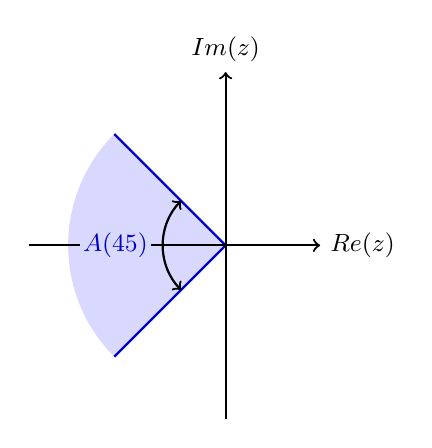
\begin{tikzpicture}

    % Parametri scalati per un grafico più piccolo
    \def\theta{45} % Ampiezza dell'angolo
    \def\R{2}      % Raggio della regione dimezzato

    % Colora la regione A(theta)
    \fill[blue!15] (0,0) -- ({180-\theta}:\R) arc ({180-\theta}:{180+\theta}:\R) -- cycle;

    % Disegna i bordi del cono
    \draw[thick, blue!80!black] (0,0) -- ({180-\theta}:\R);
    \draw[thick, blue!80!black] (0,0) -- ({180+\theta}:\R);

    % Disegna gli assi (molto più corti)
    \draw[->, thick] (-2.5, 0) -- (1.2, 0) node[right, font=\small] {$\operatorname{Re}(z)$};
    \draw[->, thick] (0, -2.2) -- (0, 2.2) node[above, font=\small] {$\operatorname{Im}(z)$};

    % Disegna gli archi per indicare l'angolo \theta (raggio ridotto)
    \draw[->, thick] (-0.8, 0) arc (180:{180-\theta}:0.8) node[midway, left=2pt, above=-1pt, font=\small] {};
    \draw[->, thick] (-0.8, 0) arc (180:{180+\theta}:0.8) node[midway, left=2pt, below=-1pt, font=\small] {};

    % Etichetta per la regione
    \node[blue!80!black] at (-1.4, 0) [fill=blue!15, inner sep=1pt, font=\small] {$A(\theta)$};

\end{tikzpicture}\\
Prendiamo in esempio l'equazione del calore
\[
\begin{cases}
	u_t = u_{xx} \ \ [0,1]\times\R^+\\
	u(x,0) = u_0(x)
\end{cases}
.\] 
$x_i = i\Delta x$ \ \  $u_{xx}(x_i)\approx \frac{u(x_{i+1}) - 2u(x_i) + u(x_{i-1})}{\Delta x^2}$  \ \ \ $O(\Delta x^2)$
 \[
	 u_t(x_i) = \frac{u(x_{i+1} - 2u(x_i) + u(x_{i-1})}{\Delta x^2} \ \ i=-,\ldots, Nx
.\] 
Eulero in tempo
\[
	\frac{u^{n+1}(x_i) - u^n(x_i)}{\Delta t} = frazione precedente
.\] 
e questo è stabile se $\frac {\Delta t}{\Delta x^2}\leq \frac 12$\\
Questo per dire che possiamo riciclare quello che sappiamo per le ODE con le PDE.
\end{document}
